\subsection{系統概述}

本小節將會介紹個別功能模組的功能、設計概念與實作方式。

%% ####################### %%
\subsubsection{登入模組}
在登入模組中需包含以下幾點功能: 
\begin{itemize}
\item{宣稱身分}
\item{身分認證}
\item{取得回傳之 token 並解構}
\end{itemize}
在宣稱身分的地方必須由使用者宣稱自己的身分並提供相關認證資料,在經由計算機中心所提供之 single sign-on 之服務完成身分認證之後,回傳給系統一組經認證的特定格式之 Token。若使用者為初次登入本系統,則此 Token 在經系統解構之後必須能夠抽取部分必要資料填入系統之資料庫中做為使用者個基礎資訊。此行為將於前端網頁系統中完成,若有需要填入時則會交由後端資料系統負責。使用者與系統之間的互動請參考圖~\ref{pic:seq:login}。

\begin{figure}[h]
\centering
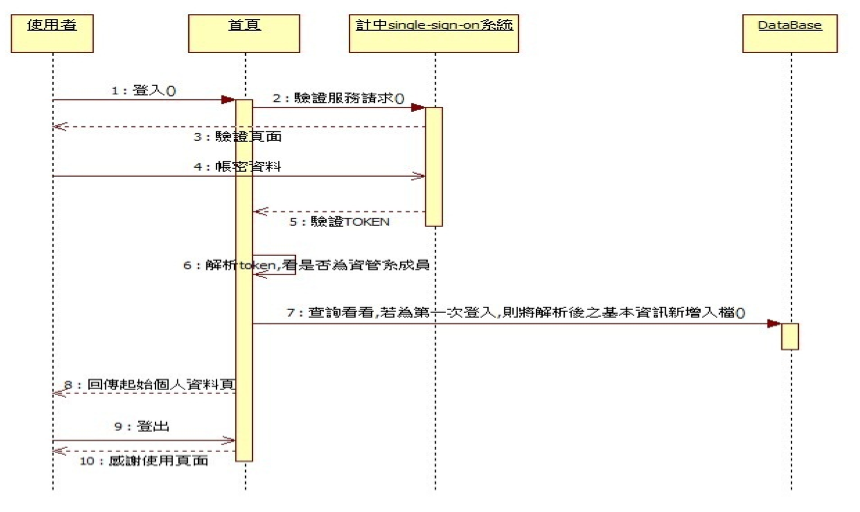
\includegraphics[width=\textwidth]{img/seq01.png}
\caption{Sequence Diagram -- 首頁登入}
\label{pic:seq:login}
\end{figure}

%% ####################### %%
\subsubsection{個人資料管理模組}
\label{sssec:userprofile}
個人資料管理模組將負責管理每個使用者各自的資料組,此資料組中包含使用者的公開資料、個人連絡資料、職業生涯相關資料與隱私權管理及關係管理。使用者必須能夠看見目前系統內的資料狀況並且能夠更動大部分的資料,其中如學號等等的則必須要經過系統管理者之認證後方可變更。此更改之行為將於前端網頁系統中完成,若有資料必須儲存則會交由後段資料系統負責。使用情境請參考圖~\ref{pic:use:userLogin},使用者與系統之間的互動請參考圖~\ref{pic:seq:login} 與圖~\ref{pic:seq:profileMgt}。

\begin{figure}[h]
\centering
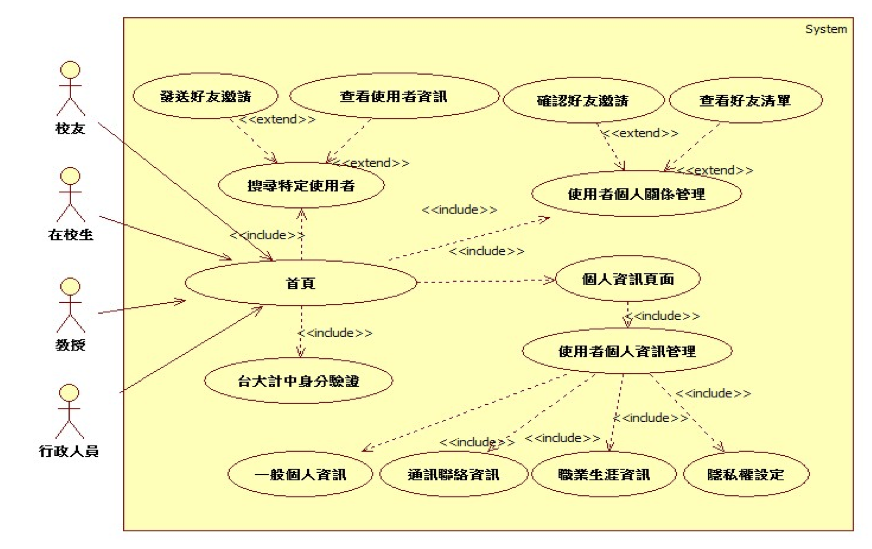
\includegraphics[width=\textwidth]{img/use01.png}
\caption{Use Case Diagram -- 使用者資訊管理}
\label{pic:use:userLogin}
\end{figure}

\begin{figure}[h]
\centering
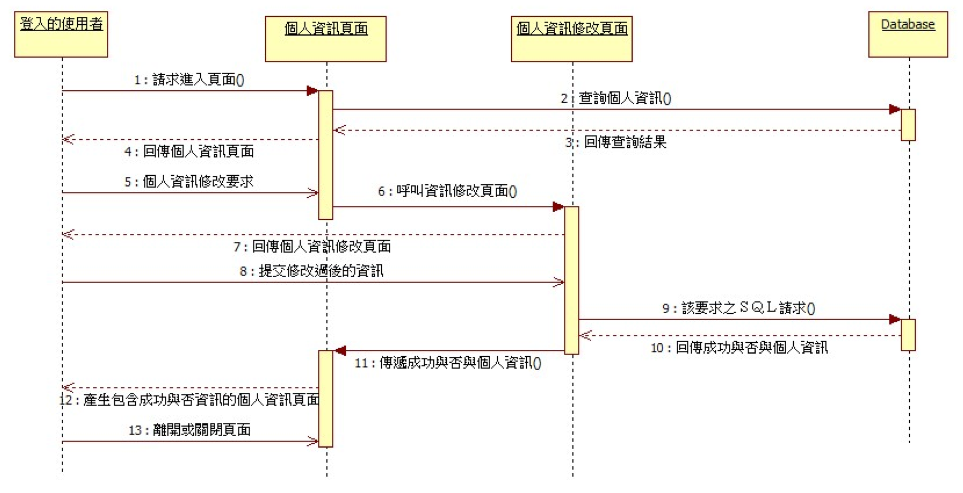
\includegraphics[width=\textwidth]{img/seq02.png}
\caption{Sequence Diagram -- 個人資訊管理與個人資訊修改}
\label{pic:seq:profileMgt}
\end{figure}

%% ####################### %%
\subsubsection{搜尋模組}
本系統為了建立一個適合使用者相互溝通之平台,必須提供使用者方便互相連結之功能,搜尋模組正是為了此需求所建立。當使用者在討論區中產生對特定用戶之好奇心,便可藉由本模組使用特定資料(如:學號)做為索引找到該用戶之公開資訊。公開程度將依該用戶之隱私設定做限制,若該用戶認為預設之帳號類別方式無法達成所欲之特殊公開之組合則需透過朋友關係的建立來達成要求。互相成為朋友的兩人將以特別規則優於普通規則的方式優先採用該用戶所設定的特別規則觀看公開資訊。本搜尋功能將全部於前端網頁系統完成。使用情境請參考圖~\ref{pic:use:userLogin},使用者與系統之間的互動模式請參考圖~\ref{pic:seq:searchUser}。

\begin{figure}[H]
\centering
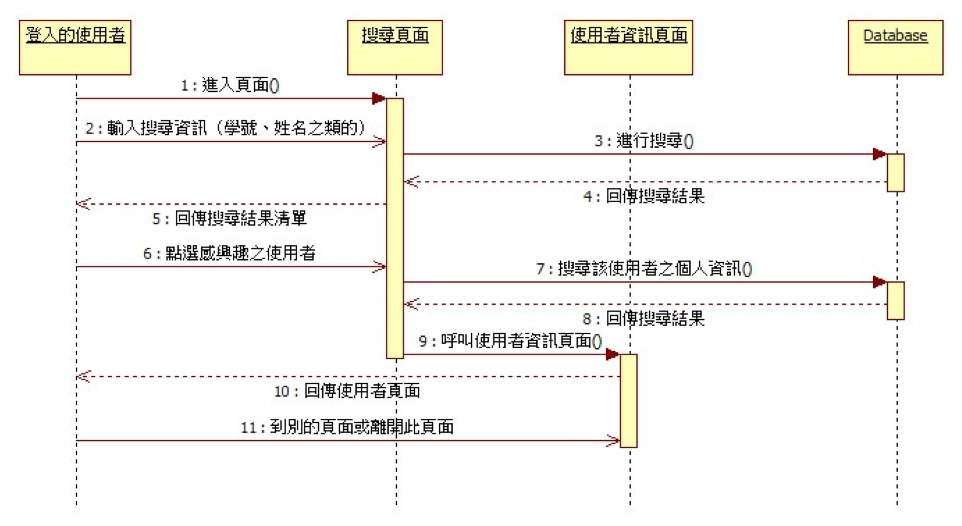
\includegraphics[width=\textwidth]{img/seq03.png}
\caption{Sequence Diagram -- 搜尋查看他人使用者資訊}
\label{pic:seq:searchUser}
\end{figure}

%% ####################### %%
\subsubsection{關係建立模組}
\label{sssec:following}
本系統中基於完成使用者之特定隱私權設計之理念,將在系統中提供建立好友關系的功能,也就是本模組的核心。本模組必須要能傳遞使用者教朋友的邀請、記錄使用者對於要求的回應與記錄使用者與其他用戶之關係。使用情境請參考圖~\ref{pic:use:userLogin}。

%% ####################### %%
\subsubsection{討論區模組}
討論區模組需包含以下幾點功能:
\begin{itemize}
\item 新增文章
\item 瀏覽文章
\item 標示文章類別
\end{itemize}
在新增文章時使用者將被要求選擇文章類別,以供其他使用者快速過濾想閱讀之訊息。由於系統沒有自動根據文章內容判斷其真實內容之能力,目前仍需仰賴使用者自動自發之行為來維持正確性,未來若能發展出足以將此行為自動化之方法則可降低系統在本問題之人力需求。此模組需同時提供標示文章類別與讓使用者方便瀏覽之功能,以達訊息交流之初衷。本模組將由前端網頁系統負責,只有將文章記錄至資料庫的行為需要後端資料系統輔助。

%% ####################### %%
\subsubsection{訂閱模組}
\label{sssec:subscription}
訂閱模組中包含訂閱使用者、訂閱文章及訂閱文章類別等三種功能。訂閱之行為一致為當訂閱之目標有了內容之新增與改變時,將由後端信件系統發信至訂閱人所登記之信箱提醒使用者。訂閱使用者的訂閱對象為本系統之其他使用者,資料的改變為新增文章等行為。訂閱文章的訂閱隊項為單篇文章,訂閱方法可包括在該文章留言或是點選訂閱按鈕,資料的改變為該文章被新增了評論時提醒。訂閱文章類別則將在任何一篇文章被標示為該類別時提醒使用者。本模組需由前端網頁系統展現、後端資料系統記錄與後端郵件系統共同合作完成。


%% ####################### %%
\subsubsection{使用者列表模組}
本模組中需要能夠條列式的顯示所有使用者之公開資料。在使用者指定過濾條件之後則依照新的過濾條件篩選資料,並將最後結果在前端網頁系統中展現給使用者。

